\documentclass[12pt,letterpaper]{article}
\usepackage[utf8]{inputenc}
\usepackage{amsmath}
\usepackage{amsfonts}
\usepackage{amssymb}
\usepackage{fancyhdr}
\usepackage{graphicx}
\usepackage[left=0.79in, right=0.79in, top=0.79in, bottom=0.79in]{geometry}
\usepackage{listings}
\usepackage[svgnames]{xcolor}
\author{Chathan Driehuys}

\definecolor{diffstart}{named}{Grey}
\definecolor{diffincl}{named}{Green}
\definecolor{diffrem}{named}{OrangeRed}

\lstset{frame=tb,
	language=html,
	aboveskip=3mm,
	belowskip=3mm,
	showstringspaces=false,
	columns=flexible,
	basicstyle={\small\ttfamily},
	breaklines=true,
	breakatwhitespace=true,
	tabsize=2
}

\graphicspath{{./images/}}

\pagestyle{fancy}
\lhead{COMP 535}
\chead{Firewall}
\rhead{Chathan Driehuys}

\begin{document}
	\noindent \textbf{UNC Honor Pledge:} I certify that no unauthorized assistance has been received or given in the completion of this work.
	
	\vspace{.5in}
	
	\section*{Prerequisites}
		In order to demonstrate the effect of firewalls, we first had to set up two virtual machines (VMs) on the same network. To prove that the two machines can exchange traffic, we can show the result of pinging one machine from another.
		
		\begin{figure}[h]
			\begin{center}
				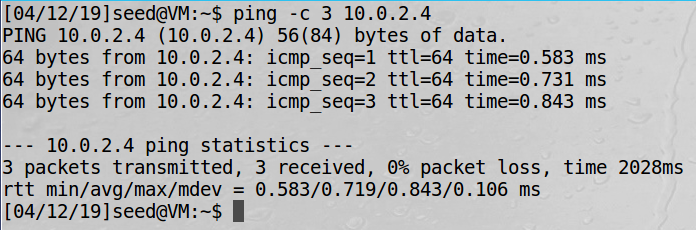
\includegraphics[width=4in]{task-0-ping}
			\end{center}
			\caption{The result of pinging one virtual machine from another.}
			\label{fig:task-0-ping}
		\end{figure}
	
	\section*{Task 1}
		Using the set of rules shown in Figure \ref{fig:task-1-ufw-rules}, we can block the following operations:
		
		\begin{enumerate}
			\item Telnet from A to B
			\item Telnet from B to A
			\item Access to \texttt{example.com} from A
		\end{enumerate}
		
		\begin{figure}
			\begin{center}
				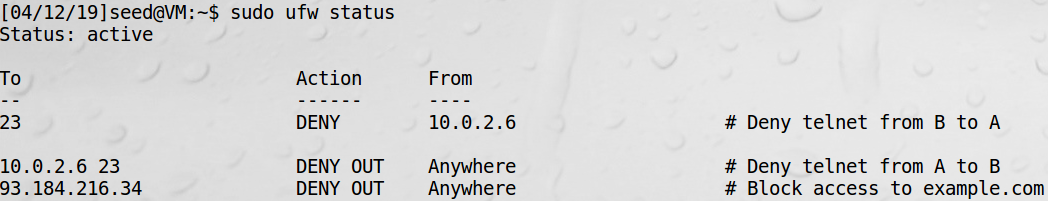
\includegraphics[width=\linewidth]{task-1-ufw-rules}
			\end{center}
			\caption{The \texttt{ufw} rules for task 1.}
			\label{fig:task-1-ufw-rules}
		\end{figure}
	
	\section*{Task 2}
		In addition to the filters from the first task, we also implemented the following rules:
		
		\begin{enumerate}
			\item Block access to \texttt{syr.edu} from A
			\item Block SSH access from B to A
		\end{enumerate}
	
		Given the template for our firewall LKM from the lab instructions, we can add the following code to the pre or post routing hook to extract some useful information about each incoming or outgoing packet.
	
		\begin{lstlisting}[caption={Extracting info from packets.}, language=c]
struct iphdr *packet_header = (struct iphdr*) sk_network_header(skb);

if (ip_header->protocol == TCP_PROTO) {
	struct tcphdr *tcp_header = (struct tcphdr*) skb_transport_header(skb);
	
	unsigned int src_ip = (unsigned int) ip_header->saddr;
	unsigned int src_port = (unsigned int) ntohs(tcp_header->source);
	unsigned int dest_ip = (unsigned int) ip_header->daddr;
	unsigned int dest_port = (unsigned int) ntohs(tcp_header->dest);
}
		\end{lstlisting}
		
		Now that we have this information, it is fairly trivial to drop packets that meet specific criteria. For example, to implement the dropping of inbound telnet packets from machine B to machine A, we would add the following code to the hook for \texttt{NF\_INET\_PRE\_ROUTING}:
		
		\begin{lstlisting}[caption={Blocking telnet traffic from machine B to machine A}]
if (src_ip == MACHINE_B_IP) && dest_port == TELNET_PORT) {
	return NF_DROP;
}
		\end{lstlisting}
		
		All the implemented rules are variations of the above code sample that inspect various combinations of the source and destination IP address and port.
		
\end{document}